\documentclass[a4paper]{article}
\usepackage{interspeech2013,amssymb,amsmath,graphicx,tipa,cite}
\setcounter{page}{1}
\sloppy		% better line breaks
\ninept
%SM below a registered trademark definition
\def\reg{{\rm\ooalign{\hfil
     \raise.07ex\hbox{\scriptsize R}\hfil\crcr\mathhexbox20D}}}


\makeatletter
\def\bstctlcite{\@ifnextchar[{\@bstctlcite}{\@bstctlcite[@auxout]}}
\def\@bstctlcite[#1]#2{\@bsphack
  \@for\@citeb:=#2\do{%
    \edef\@citeb{\expandafter\@firstofone\@citeb}%
    \if@filesw\immediate\write\csname #1\endcsname{\string\citation{\@citeb}}\fi}%
  \@esphack}
\makeatother


%% \newcommand{\reg}{\textsuperscript{\textcircled{\textsc r}}}
\title{The effects of stress/accent on VOT depend on language (English, Spanish), consonant (/d/, /t/) and linguistic experience (monolinguals, bilinguals)}

\makeatletter
\def\name#1{\gdef\@name{#1\\}}
\makeatother
\name{{\em Miquel Simonet, Joseph V. Casillas, Yamile D\'{i}az}}

\address{Department of Spanish \& Portuguese \\ University of Arizona, Tucson, Arizona U.S.A.\\
{\small \tt \{simonet,jvcasill,ydiaz44\}@email.arizona.edu}}

\begin{document}
\bstctlcite{IEEEexample:BSTcontrol}
\maketitle
%
\begin{abstract}
This study examines Voice Onset Times of coronal stops in utterance-initial position in two languages. Crucially, the effects of lexical stress (stressed, unstressed syllable) on VOT are analyzed. The study investigates aspirated stops (English /t/), short-lag voiceless stops (English /d/, Spanish /t/) and prevoiced stops (Spanish /d/). Three groups of speakers provide data: English monolinguals, Spanish monolinguals, and proficient Spanish-English bilinguals. The study finds that lexical stress lengthens aspiration (English /t/) and prevoicing (Spanish /d/) but it does not alter significantly short-lag stops (Spanish /t/, English /d/). Monolinguals and bilinguals differ slightly in their phonetic behavior. Implications for gestural coordination as well as for feature theory are discussed.
\end{abstract}
\noindent{\bf Index Terms}: VOT, stress, Spanish, English, bilingualism



%
\section{Introduction}

The present study is concerned with the effects of lexical stress on Voice Onset Times (VOT) of /d/ and /t/ in two languages, Spanish and English. The study examines the productions of monolingual and bilingual speakers and assesses the potential impact of linguistic experience on lexical stress effects for Spanish and English /d/ and /t/.

While both Spanish and English possess a contrast between \emph{fortis} (/p t k/) and \emph{lenis} stops (/b d g/), the phonetic implementation of the contrast differs for the two languages. English presents a contrast between a set of aspirated, voiceless stops (/p t k/) and a set of unaspirated, voiceless stops (/b d g/). The Spanish contrast is that between a set of unaspirated, voiceless stops (/p t k/) and a set of voiced stops (/b d g/) \cite{rosner2000voice}. (Note that this description applies to utterance-initial position because Spanish /b d g/ are regularly spirantized in other positions). According to one view, the phonological opposition in English depends on the feature [spread glottis], which is specified for the \emph{fortis} stops but not for the \emph{lenis} ones; on the other hand, the Spanish contrast depends on [voice], which is specified for the \emph{lenis} stops but not for the \emph{fortis} ones \cite{beckman2011rate}.

A large body of research has demonstrated that prosodic structure affects fine-phonetic detail in segments. Experimental studies have shown that consonants in prominent syllables (stressed, accented) are hyperarticulated relative to those in non-prominent syllables (unstressed, unaccented) in a number of languages (\cite[among others]{cho2009effects, cho2005prosodic, Cole:2003uq, de-Jong-Ken:1995fk, Abramson:1967fk}). Hyperarticulation is captured by articulatory and acoustic measurements. One of the acoustic correlates that manifest hyperarticulation is VOT. In a seminal study, \cite{Abramson:1967fk} found that VOTs in English aspirated stops (/p t k/) were longer when these consonants were found at the onset of lexically stressed syllables than when they were found at the onset of unstressed syllables. This effect was corroborated, for this language, in \cite{cho2009effects} and, for phrase-accented syllables in connected speech, in \cite{Cole:2003uq}. In sum, for consonants with long-lag VOT, such as English /p t k/, the effects of lexical stress are straightforward, and they seem to be of an additive nature---stress lengthens the aspiration period of aspirated consonants.

Stress effects also have been investigated for consonants with short-lag VOTs, although the results are less straightforward than those for aspirated consonants \cite{Castaneda:1986eu, Poch:1985bv, Troya:2005hh}. For instance, \cite{Abramson:1967fk} reported a trend for English /b d g/ according to which these consonants showed a \emph{shorter} VOT when stressed than when unstressed. On the other hand, \cite{Cole:2003uq}'s findings are not in line with those in \cite{Abramson:1967fk} regarding English /b d g/. In \cite{Cole:2003uq}'s study, VOT is lengthened when the consonant bears prominence, and that applies to both /p t k/ (English aspirated stops) as well as to /b d g/ (English short-lag, unaspirated stops). The results of a study of Dutch \emph{fortis} (/t/) and \emph{lenis} (/d/) stops are also informative in this regard \cite{cho2005prosodic}. Dutch presents a \emph{fortis-lenis} contrast of the ``Spanish type'', rather than the ``English type''; that is, Dutch /t/ is a voiceless, unaspirated stop---a stop with a short-lag VOT. \cite{cho2005prosodic} explores the effects of lexical stress and phrasal accent separately. In this study, VOT length of Dutch /t/ is longest when unstressed and unaccented and shortest when stressed and accented. Thus, the effects of stress on this consonant are subtractive (in terms of VOT), rather than additive, and the effects of lexical stress and phrasal accent are cumulative.

No study seems to have straightforwardly addressed the effects of lexical stress on negative VOT or prevoiced stops \cite[cf.]{Castaneda:1986eu, Poch:1985bv}. \cite{cho2005prosodic} analyzed the duration of voicing during closure in Dutch /d/. In the data in this study, /d/ always appeared in intervocalic, rather than utterance-initial, position. Although this measurement might differ from lead VOT (since voicing during closure in intervocalic /d/ could be due partially to carryover laryngeal coarticulation), the findings in \cite{cho2005prosodic} with respect to /d/ are perhaps relevant---lexical stress was found to affect voicing length. In particular, prominent syllables displayed longer voicing periods during closure than unstressed syllables. The fact remains that, to our knowledge, the effects of stress on prevoiced stops remains to be investigated in depth.

The present study analyzes lexical stress effects on long-lag stops (English /t/), short-lag stops (English /d/, Spanish /t/) and prevoiced stops (Spanish /d/). Thus, we explore a language with a [spread glottis] contrast (English), one with a [voice] contrast (Spanish), and, importantly, we study speakers possessing both features and thus all three stop types (Spanish-English bilinguals). The goal of the present study is to gain a broader understanding of stress effects on different VOT categories in order to begin to grasp the impact of prosody on segments more generally.

\section{Methods}

In order to collect the production data, we used a delayed shadowing task, widely used in the literature on second-language speech learning (e.g., \cite{guion2003vowel}). In this task, speakers listen to and then repeat out loud target phrases.

\subsection{Materials}

\subsubsection{Target phrases}

The materials were a list of words beginning with /d/ or /t/. Half of these words were stressed on the word-initial syllable, and the other half were stressed on the second syllable. Therefore, stops could appear in a stressed syllable or unstressed syllable. There were 40 words total, 20 per language. The words were balanced for Consonant (/d/, /t/) and Stress (stressed, unstressed). There were five word items per design cell: 2 (languages) $\times$ 2 (consonants) $\times$ 2 (stress configurations) = 8 design cells $\times$ 5 items = 40 words. The target words were interspersed among many fillers or distractors (\emph{n} = 36).

\subsubsection{Auditory stimuli}

The 40 words were printed out on two lists as a function of language---20 English and 20 Spanish words. Three male native speakers of each language (six `talkers' in total) were asked to read their corresponding word list out loud. Each `talker' received a different randomization of the list. Words were produced in utterance-initial position in the carrier sentences `\_\_ is the word' and `\_\_ es la palabra.' In this way, three auditory models were recorded for each word item, one per `talker.' This amounted to 120 (20 items $\times$ 2 languages $\times$ 3 auditory models or `talkers') different auditory stimuli to be used in the delayed shadowing task. 

\subsection{Speakers}

A total of 47 volunteers participated in this experiment. All speakers were female, and they were all between 18 and 23 years of age. There were three groups of speakers: (i) a group of Spanish-English bilinguals (\emph{n} = 19), (ii) a group of monolingual Spanish speakers (\emph{n} = 22), and (iii) a group of monolingual English speakers (\emph{n} = 7). The monolingual Spanish speakers were recruited from among the student body of the Universitat de les Illes Balears on Majorca, Spain. These participants are bilingual in Catalan. (Note that there are no reported differences between Catalan and Spanish stop consonants with respect to their VOT \cite{amengual2012interlingual}.) The monolingual English speakers, as well as the Spanish-English bilinguals, are/were undergraduate students at the University of Arizona in Tucson, Arizona. The English speakers consider English to be their native language, and they were exposed to English exclusively in their family circle while growing up. The bilinguals, Mexican-Americans born and raised in Southern Arizona, were brought up by Spanish-speaking families and were schooled mostly in English. They use both languages daily both in the classroom as well as with their friends and relatives. A bilingual profile questionnaire was used to establish the groups \cite{birdsong2012bilingual}. In this report, data from the three groups are analyzed separately.  

The Spanish-English bilinguals were recorded in both of their languages. The English monolinguals were recorded in English. The Spanish monolinguals were recorded in Spanish.

\subsection{Procedure}

The 47 female speakers were asked to listen to and then repeat out loud the auditory stimuli. The English monolinguals heard and produced only the English materials (60 tokens). The Spanish monolinguals heard and produced only the Spanish materials (60 tokens). The Spanish-English bilinguals, however, were recorded in both of their languages---they listened to and repeated the English as well as the Spanish materials (120 tokens). Each speaker heard a different randomization of the stimuli.

Importantly, the bilinguals heard and produced the English and Spanish materials in a single block, in random order. In other words, the Spanish and English auditory stimuli were randomized in one single production session so that the English items were interspersed amongst the Spanish items. This hypothetically maximizes the degree of interlingual transfer of phonetic characteristics for these bilinguals \cite{olson2013bilingual}, and it thus explores this population in a situation diametrically opposed to the one researched in \cite{magloire1999cross}. Speakers were asked to listen to the entire utterance first (`\_\_ is the word' or/and `\_\_ es la palabra') and then to repeat the entire sequence aloud. In this way, shadowing of the target consonant was slightly delayed relative to the time in which it was heard.

Recordings were made through a head-mounted dynamic microphone (Shure SM10A), a pre-amp (Sound Devices MM-1) and a digital voice recorder (Marantz PMD660). Digitization was at 44.1 kHz, 16-bit. The Spanish monolinguals were recorded in a quiet laboratory at the Universitat de les Illes Balears. The English monolinguals and the Spanish-English bilinguals were recorded in a sound-attenuated booth at the Applied Phonetics Laboratory of the University of Arizona. Speakers were recorded one at a time.

\subsection{Analysis}

A total of 4,020 word tokens were collected for the present study. The English speakers provided 420 tokens, the Spanish speakers provided 1,320 tokens, and the Spanish-English bilinguals provided 2,280 tokens, 1,140 in Spanish and 1,140 in English. The study considered two within-speaker factors: (i) Consonant: /d/, /t/; and (ii) Stress: first syllable in word is either stressed or unstressed. For one of the speaker groups (Spanish-English bilinguals) a third within-speaker factor was added---Language spoken: Spanish, English.

The target /d/ and /t/ tokens were measured for VOT \cite{lisker1963crosslanguage}. VOT is an acoustic metric that captures, for stops, the time lag between the burst (i.e., the release of the articulators after the stop closure) and the initiation of periodicity (i.e., the onset of modal voicing). VOT is positive if the burst occurs before the onset of periodicity (since burst = 0 ms) and negative if it occurs after it. In this study, bursts and voicing onsets were hand-located by exploring spectrographic and sound wave displays. The onset of voicing was marked at a zero-crossing on a sound wave display. Voicing onset in lag VOTs was marked by taking into account the initiation of $F2$ in order to make sure that we labeled the initiation of modal voicing rather than voicing \emph{per se}.

\section{Results}

\subsection{Spanish speakers}

The Spanish materials produced by the Spanish speakers were analyzed through a repeated-measures ANOVA with VOT (ms) as the dependent variable and Consonant (/t/, /d/) and Stress (stressed, unstressed) as within-subjects factors. Individual speaker (\emph{n} = 22) was the error term. The descriptive statistics of these data are shown in Table \ref{tab:span}. The statistical test revealed significant effects of Consonant ($F(1,21) = 511.7, p < 0.001$) and Stress ($F(1,21) = 123, p < 0.001$), as well as a two-way significant interaction ($F(1,21) = 135.7, p < 0.001$). For these Spanish speakers, /d/ has a lead, negative VOT with a mean of -59.8 ms and /t/ has a short-lag, positive VOT with a mean of 15.8 ms.

\begin{table}
	\centering
	\begin{tabular}{|l|c|c|}
	\hline
	& /d/ & /t/ \\
	\hline \hline
	stressed & -69.2 (3.52) & 15.3 (1.04) \\
	unstressed & -50.4 (3.51) & 16.3 (1.38) \\
	\hline
	\end{tabular}
		\caption{Mean (+ SE) VOT (ms) as a function of Consonant (/t/, /d/) and Stress (stressed, unstressed) in the Spanish data.} \label{tab:span}
\end{table}

In order to explore the interaction, the main effects of Stress were investigated for the two stop consonants separately; this was done by means of paired t-tests. The alpha level was adjusted accordingly (0.05/2 = 0.025) On the one hand, /d/ was shown to present longer prevoicing when stressed than when unstressed by a factor of 1.373 ($t(21) = -12.02, p < 0.001$). On the other hand, /t/ was found not to be affected by Stress ($t(21) = -1.85, p > 0.05$).

\subsection{English speakers}

The English VOT data were explored by means of a repeated-measures ANOVA with Consonant (/t/, /d/) and Stress (stressed, unstressed) as main factors. Subject (\emph{n} = 7) was the Error term. The ANOVA yielded significant Consonant effects ($F(1,6) = 244.9, p < 0.001$), but no significant effects of Stress ($F(1,6) = 1.27, p > 0.05$). The model revealed a significant two-way interaction ($F(1,6) = 19.22, p < 0.01$). Descriptive statistics are provided in Table \ref{tab:eng}.

\begin{table}
	\centering
	\begin{tabular}{|l|c|c|}
	\hline
	& /d/ & /t/ \\
	\hline \hline
	stressed & 21.9 (3.66) & 78.4 (6.72) \\
	unstressed & 26.3 (4.81) & 71.4 (5.89) \\
	\hline
	\end{tabular}
		\caption{Mean (+ SE) VOT (ms) as a function of Consonant (/t/, /d/) and Stress (stressed, unstressed) in the English data.} \label{tab:eng}
\end{table}

The interaction was examined by means of two separate paired t-tests, and the alpha level was adjusted accordingly. The interaction was due to the fact that Stress effects were robust for /t/ ($t(6) = 3.8, p < 0.01$), but not for /d/ ($t(6) = -2.7, p = 0.03$). At most, one could claim that a marginal trend exists for /d/ as well, although in the opposite direction. The effects for /t/ were due to the fact that stressed /t/ displays a longer period of aspiration than unstressed /t/ by a factor of 1.098.

\subsection{Spanish-English bilinguals}

The bilingual VOT data were submitted to a repeated-measures ANOVA with Language (Spanish, English), Consonant (/t/, /d/) and Lexical Stress (stressed, unstressed) as fixed factors. All these were within-subjects factors since bilinguals were recorded in both languages. Subject (\emph{n} = 19) was the error term. The statistical model yielded significant effects of all three main effects: Language ($F(1,18) = 249.5, p < 0.001$), Consonant ($F(1,18) = 152.4, p < 0.001$), and Stress ($F(1,18) = 7.58, p = 0.01$). More relevant was the fact that the model revealed three significant two-way interactions (Consonant by Language, $F(1,18) = 5.3, p = 0.03$; Language by Stress, $F(1,18) = 54.5, p < 0.001$; Consonant by Stress, $F(1,18) = 16.95, p < 0.001$) and a significant three-way interaction ($F(1,18) = 31.6, p < 0.001$). In order to explore the interactions, the dataset was divided into subsets.

Firstly, the effects of Consonant and Stress were examined for the two languages separately. The first ANOVA investigated the effects of these two fixed, within-subjects factors on VOT for the English data only. These data are plotted in Figure \ref{fig:eng}. This model yielded significant effects of Consonant ($F(1,18) = 140, p < 0.001$), as well as Stress ($F(1,18) = 17.3, p < 0.001$). Importantly, there was no interaction between the two factors ($F(1,18) < 1$). The effects of Stress were due to the fact that stressed consonants had a longer VOT (a VOT further away from zero) than unstressed consonants by a factor of 1.18. Note that both consonants (/t/, /d/) were similarly affected by the effects of stress in this data subset.

	\begin{figure}
		\centering
		\caption[English]{Effects of lexical stress on VOT in English /t/ and /d/ in the bilingual speakers' productions. \label{fig:eng}}
		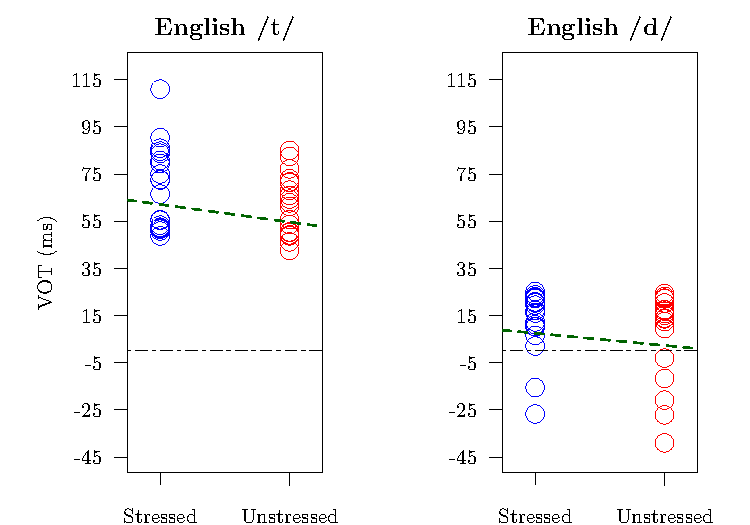
\includegraphics[width=70mm]{figures/bil_eng.pdf}
	\end{figure}

	\begin{figure}
		\centering
		\caption[English]{Effects of lexical stress on VOT in Spanish /t/ and /d/ in the bilingual speakers' productions. \label{fig:span}}
		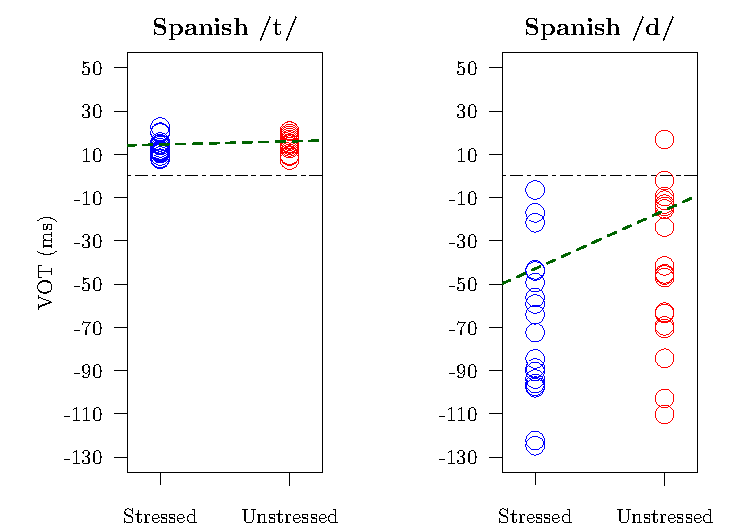
\includegraphics[width=70mm]{figures/bil_sp.pdf}
	\end{figure}

The second follow-up ANOVA explored the effects of Consonant and Stress for the Spanish materials only. (See Figure \ref{fig:span}.) In this analysis, Consonant and Stress were within-subjects factors and speaker was the error term. The model revealed significant effects of Consonant ($F(1,18) = 99.25, p < 0.001$) and Stress ($F(1,18) = 35.38, p < 0.001$), as well as a significant two-way interaction ($F(1,18) = 28.42, p < 0.001$). The interaction was due to the fact that /d/ was affected by Stress ($t(18) = -5.73, p < 0.001$) while /t/ was not ($t(18) = -1.6, p > 0.1$). In these data, stressed /d/ had longer prevoicing than unstressed /d/ by a factor of 1.63.

\section{Discussion and conclusions}

The present study has reported on the results of a production experiment in which the effects of lexical stress on VOT length are examined. VOTs were measured for /d/ and /t/ in both Spanish and English. Three groups of speakers were recorded: Spanish and English monolinguals, and Spanish-English bilinguals. The three groups were investigated separately.

Regarding English /d/ and /t/, the study found that the \emph{fortis}, aspirated stop (/t/) was affected by stress while the \emph{lenis} stop (/d/) was not (or marginally so). The effects of stress on English /t/ were additive---lexical stress lengthened aspiration in this consonant. Therefore, it could be said that stress enhances the acoustic difference between the two members of the /d/-/t/ contrast by affecting one of the two.

The situation for Spanish was different from that for English. In Spanish, it was the \emph{lenis} stop (/d/), rather than the \emph{fortis} one (/t/), the one to be impacted by lexical stress. Spanish /t/ was not modulated by stress. The effects of stress on Spanish /d/ were straightforward---stress lengthens prevoicing in this consonant. Once again, therefore, it could be claimed that stress enhances the acoustic opposition between /d/ and /t/ by displacing one of the two members of the contrast.

The findings of the present study regarding the effects of lexical stress on three VOT categories of two different languages are reminiscent of the literatures on the effects of (i) clear speech and (ii) of speech rate on these sound categories. For instance, \cite{smiljanic2008clear} found that, in clear speech, aspiration is lengthened in English \emph{fortis} stops and prevoicing is lengthened in Croatian \emph{lenis} stops---short-lag VOT categories are largely unaffected by clear speech.

With respect to speech rate effects, studies typically find that as speech rate decreases (i.e., speech becomes slower) VOTs lengthen, but not for all stop consonants \cite{allen1999vot,kessinger1997vot}. In parallel to the studies on clear speech (and stress effects), the literature on speech rate has shown that aspiration is lengthened in English \emph{fortis} stops while VOT is not impacted (or only minimally so) in stops characterized by short-lag VOTs \cite{allen1999vot}. In a fundamental cross-linguistic study, \cite{kessinger1997vot} researched the effects of speech rate on Thai, French and English stops. French has a contrast of the ``Spanish-type''---\emph{fortis} stops are voiceless, unaspirated and \emph{lenis} stops are prevoiced. Thai has a three-way contrast---it possesses sets of (i) voiceless, aspirated stops, (ii) voiceless, unaspirated stops, and (iii) prevoiced stops. The study found that slow speech lengthened aspiration in English \emph{fortis} stops and French \emph{lenis} stops while short-lag VOT (English \emph{lenis}, French \emph{fortis}) stops were not affected. Regarding the case of Thai, the study found that short-lag VOT categories were not modulated by speech rate while the other two VOT categories were---VOTs were lengthened in the predictable directions.

A review of the literature suggests that the effects of speech rate, clear speech and lexical stress on VOT categories are very similar. What these studies have in common is that they find that, in two-way contrasts, short-lag VOT categories are unaffected while the other category is affected. In three-way contrasts, short-lag VOT categories are also the ones that remain largely unmodified. This could be summarized with the statement that short-lag VOT stop categories act as anchors in situations that lead to contrast enhancement, such as slow and/or clear speech and prosodic prominence. 

The ``contrast-enhancement'' perspective, however, has been challenged by a study that investigated the effects of speech rate on Central Standard Swedish \cite{beckman2011rate}. This language has a two-way contrast. It opposes a set of aspirated, voiceless stops with a set of prevoiced stops---a short-lag VOT category is not found in this language. In Swedish, both stop consonants are affected by slow speech. In sum, the same categories that are affected in French, English and Thai are also affected in Swedish---the only difference is that Swedish does not have an ``anchor''. The reasoning in \cite{beckman2011rate} is that the Swedish contrast is already acoustically large in faster speech and does not need to be enhanced. \cite{beckman2011rate} propose that speech rate, together with clear speech (and lexical stress), affects VOT categories that \emph{are specified for a phonological feature}. In this view, aspirated stops are specified for [spread glottis], prevoiced stops are specified for [voice] and, importantly, short-lag VOT stops are left unspecified. Contrast enhancement is viewed as an artifact of feature modulation.

An alternative view that does not exploit feature theory is one that depends on articulatory gesture coordination. The VOT metric measures the time lag between two acoustic events that stand for two articulatory gestures, a laryngeal and a supralaryngeal gesture. As such, the VOT metric is a measure of gesture coordination. It is possible that speech rate, clear speech and prosodic prominence do not affect gestural coordination patterns for sounds whose two gestures are robustly synchronized (short-lag VOT stops), but do for those that are loosely synchronized (prevoiced and aspirated stops).

An analysis of the bilingual data found the following: (i) Spanish /d/ is robustly affected by lexical stress while Spanish /t/ is not, and (ii) both English consonants are slightly affected by lexical stress. Therefore, for these bilingual subjects, consonants with lead VOT (Spanish /d/) and long-lag VOT (English /t/) are impacted by lexical stress, although the former more so than the latter. This is the same result that was found for the native English- and Spanish-speaking groups. From the two short-lag VOT consonant (Spanish /t/, English /d/), only English /t/ is affected by lexical stress. While English monolinguals did not display robust stress effects on their English /d/, the bilinguals did.

A possible interpretation of the bilingual findings is suggested by the fact that a subgroup of the Spanish-English bilinguals produced English /d/s with some prevoicing---see Figure \ref{fig:eng}. This could be a transfer effect from Spanish /d/ for this subgroup. Since negative VOT in prevoiced stops is indeed affected by lexical stress (Spanish /d/, for instance) it is perhaps not surprising that English /d/, as produced by this particular group, is somewhat modulated by stress. Alternatively, English, but not Spanish, \emph{lenis} stops, in general, could be impacted by lexical stress in this population. A strong interpretation of the ``featural specification hypothesis'' of \cite{beckman2011rate}, according to which only consonants with specified features are affected by prosodic modulations, is therefore not possible for the bilingual group. It could be concluded that the Spanish-English bilinguals in this study posess a phonological system consisting of [voice] (Spanish /d/), $\emptyset$ (Spanish /d/), and [spread glottis] (English /t/). The nature of the English \emph{lenis} stop would deserve more attention. If [voice] were to be chosen as the featural specification for English /d/, the question arises as to why the phonetic facts for this consonant differ from those for Spanish /d/.

\section{Acknowledgments}
The authors wish to express their gratitude to the following: Mark Amengual, Melinda Porta, Olivia Obeso, Miquel Llompart, and the 47 volunteers who participated in the study. The authors are also grateful to three anonymous reviewers, and to the SP-7 audience, for constructive criticism.

\newpage
%
\eightpt
\bibliographystyle{IEEEtran} 
\bibliography{IEEEabrv,SpeePros}{}

\end{document}
